\section{What is the confusion matrix?}
A confusion matrix is a table that is used to evaluate the performance of a binary classification model by comparing the predicted and actual class labels of a set of test data. The confusion matrix displays the number of true positives, true negatives, false positives, and false negatives made by the model.

In a binary classification problem, there are two possible classes: positive and negative. The four possible outcomes of a binary classification are:

1. True Positive (TP): the model correctly predicted a positive sample
2. True Negative (TN): the model correctly predicted a negative sample
3. False Positive (FP): the model incorrectly predicted a positive sample (also known as a Type I error)
4. False Negative (FN): the model incorrectly predicted a negative sample (also known as a Type II error)

The confusion matrix is a table that shows the number of samples that fall into each of these four categories. The rows of the matrix represent the actual class labels, while the columns represent the predicted class labels. A confusion matrix for a binary classification problem typically looks like this:

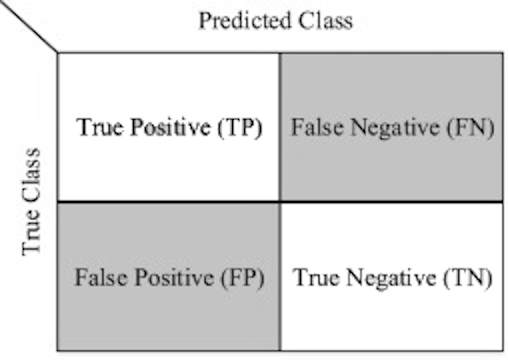
\includegraphics{./confisionmatrix}

The confusion matrix provides a detailed breakdown of the performance of the model and can be used to calculate several performance metrics, including accuracy, precision, recall, and F1 score. For example, accuracy can be calculated as (TP + TN) / (TP + TN + FP + FN), precision can be calculated as TP / (TP + FP), and recall can be calculated as TP / (TP + FN).

The confusion matrix is a useful tool for evaluating the performance of a binary classification model and can be used to identify the types of errors made by the model and to improve its performance.

